
\documentclass{article}


\usepackage{amsmath}
\usepackage{amssymb}
\usepackage{graphicx}

\graphicspath{ {./images/} }

\setlength{\parskip}{0.5\baselineskip plus2pt minus2pt}
\setlength\parindent{0pt}
\setlength{\textheight}{9in}

\title{WS3 Exam presentation}

\begin{document}
\section{Del 1}
\subsection{Delopgave 1.3}
Omskriv problemet (3) til et line\ae rt problem i kanonisk form, og bestem det duale problem.

(3):
\begin{equation}
    \begin{array}{ll}
        \text{minimize}   & \tilde{c} \cdot \tilde{x} \\
        \text{subject to} & \tilde{A}\tilde{x} = b, \\
                          & \tilde{x} \geq 0
    \end{array}
\end{equation}

\begin{equation}
    \begin{array}{ll}
        \text{maximize}   & c \cdot x \\
        \text{subject to} & Ax \leq b \\
                          & x \geq 0
    \end{array}
\end{equation}

\begin{equation}
    \tilde{A}\tilde{x} = b \implies
    \begin{bmatrix}
        \tilde{A} \\
        -\tilde{A}
    \end{bmatrix}
    \tilde{x} \leq
    \begin{bmatrix}
        b \\
        -b
    \end{bmatrix}
\end{equation}

\begin{equation}
    \hat{A} =
    \begin{bmatrix}
        \tilde{A} \\ -\tilde{A}
    \end{bmatrix},
    \hat{b} =
    \begin{bmatrix}
        b \\ -b
    \end{bmatrix}
\end{equation}

The primal problem
\begin{equation}
    \begin{array}{ll}
        \text{maximize}   & -\tilde{c} \cdot x \\
        \text{subject to} & \hat{A}\tilde{x} \leq \hat{b} \\
                          & \tilde{x} \geq 0
    \end{array}
\end{equation}

The dual problem

\begin{equation}
    \begin{array}{ll}
        \text{minimize}   & \hat{b} \cdot y \\
        \text{subject to} & \hat{A}^Ty \geq -\tilde{c} \\
                          & y \geq 0
    \end{array}
\end{equation}

\subsection{Delopgave 4}
Antag at $m = 1$, $n = 5$, $A = [1,2,3,4,5]$, $b=[10]$. Ved hj\ae lp af en tegning find en l\o sning til det duale problem I har bestemt i det sidste sp\o rsm\aa l. Brug st\ae rk dualitet til at bestemme en l\o sning til det primale problem ud fra l\o sningen til det duale. L\o s ogs\aa\ det primale problem vha. simplexmetoden, og tjek at I f\aa r samme resultat.

\begin{equation}
    \hat{b} \cdot y =
    \begin{bmatrix}
        10 \\
        -10
    \end{bmatrix}
    \cdot
    \begin{bmatrix}
        y_1 \\
        y_2
    \end{bmatrix}
    =
    10y_1 - 10y_2
\end{equation}

\begin{equation}
    \tilde{A} =
    \begin{bmatrix}
        1 & 2 & 3 & 4 & 5 & -1 & -2 & -3 & -4 & -5
    \end{bmatrix}
\end{equation}

\begin{equation}
    \hat{A} =
    \begin{bmatrix}
        1 & 2 & 3 & 4 & 5 & -1 & -2 & -3 & -4 & -5 \\
        -1 & -2 & -3 & -4 & -5 & 1 & 2 & 3 & 4 & 5
    \end{bmatrix}
\end{equation}

\begin{equation}
    \hat{A}^T =
    \begin{bmatrix}
        1 & -1 \\
        2 & -2 \\
        3 & -3 \\
        4 & -4 \\
        5 & -5 \\
        -1 & 1 \\
        -2 & 2 \\
        -3 & 3 \\
        -4 & 4 \\
        -5 & 5
    \end{bmatrix}
\end{equation}

\begin{equation}
    \hat{A}^Ty =
    \begin{bmatrix}
        1 & -1 \\
        2 & -2 \\
        3 & -3 \\
        4 & -4 \\
        5 & -5 \\
        -1 & 1 \\
        -2 & 2 \\
        -3 & 3 \\
        -4 & 4 \\
        -5 & 5
    \end{bmatrix}
    \cdot
    \begin{bmatrix}
        y_1 \\
        y_2
    \end{bmatrix}
    \geq
    \begin{bmatrix}
        -1 \\
        -1 \\
        -1 \\
        -1 \\
        -1 \\
        -1 \\
        -1 \\
        -1 \\
        -1 \\
        -1
    \end{bmatrix}
    =
    -\tilde{c}
\end{equation}

\begin{figure}[h]
    \centering
    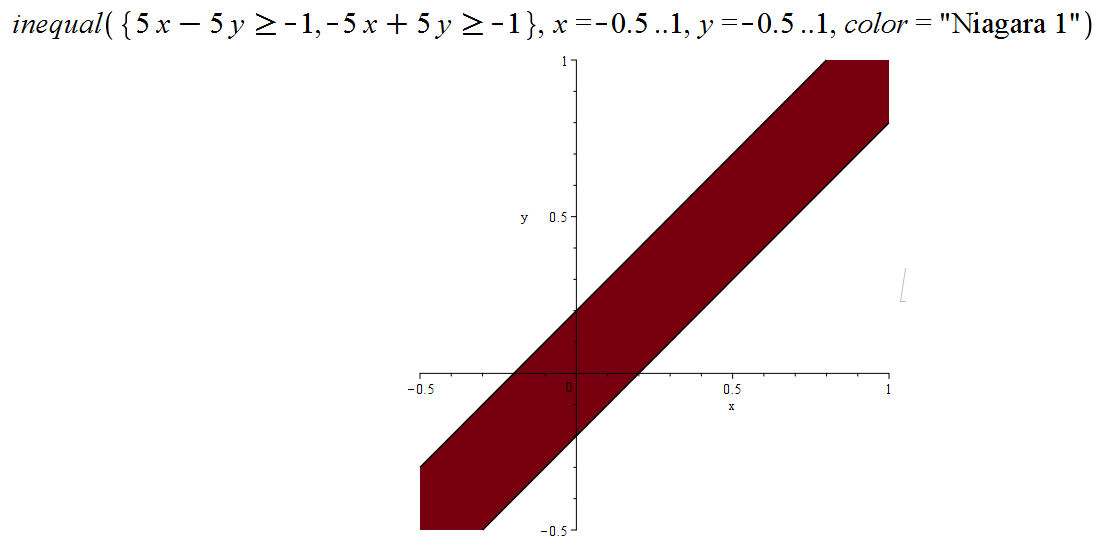
\includegraphics[width=\textwidth]{plot}
\end{figure}

\begin{equation}
    \begin{array}{ll}
        (0,0) & \implies 10 \cdot 0 - 10 \cdot 0 = 0 \\
        (0,0.2) & \implies 10 \cdot 0 - 10 \cdot 0.2 = -2 \\
        (0.2,0) & \implies 10 \cdot 0.2 - 10 \cdot 0 = 2
    \end{array}
\end{equation}

\begin{equation}
    \begin{array}{c}
        c^T\bar{x} = b^T\bar{y} \\
        -\tilde{c}^T\tilde{x} = \hat{b}^Ty = -2
    \end{array}
\end{equation}

\begin{equation}
    \begin{array}{|c|c|c|c|c|c|c|c|c|c|c|c|c|c|c|}
        \hline
        & x_1 & x_2 & x_3 & x_4 & x_5 & x_6 & x_7 & x_8 & x_9 & x_{10} & s_1 & s_2 & M & b \\
        \hline
        s_1 & 1 & 2 & 3 & 4 & 5 & -1 & -2 & -3 & -4 & -5 & 1 & 0 & 0 & 10 \\
        \hline
        s_2 & -1 & -2 & -3 & -4 & -5 & 1 & 2 & 3 & 4 & 5 & 0 & 1 & 0 & -10 \\
        \hline
        M & 1 & 1 & 1 & 1 & 1 & 1 & 1 & 1 & 1 & 1 & 0 & 0 & 1 & 0 \\
        \hline
    \end{array}
\end{equation}

\begin{equation}
    \begin{array}{|c|c|c|c|c|c|c|c|c|c|c|c|c|c|c|}
        \hline
        & x_1 & x_2 & x_3 & x_4 & x_5 & x_6 & x_7 & x_8 & x_9 & x_{10} & s_1 & s_2 & M & b \\
        \hline
        s_1 & 1 & 2 & 3 & 4 & 5 & -1 & -2 & -3 & -4 & -5 & 1 & 0 & 0 & 10 \\
        \hline
        x_5 & .2 & .4 & .6 & .8 & 1 & -.2 & -.4 & -.6 & -.8 & -1 & 0 & -.2 & 0 & 2 \\
        \hline
        M & 1 & 1 & 1 & 1 & 1 & 1 & 1 & 1 & 1 & 1 & 0 & 0 & 1 & 0 \\
        \hline
    \end{array}
\end{equation}

\begin{equation}
    \begin{array}{|c|c|c|c|c|c|c|c|c|c|c|c|c|c|c|}
        \hline
        & x_1 & x_2 & x_3 & x_4 & x_5 & x_6 & x_7 & x_8 & x_9 & x_{10} & s_1 & s_2 & M & b \\
        \hline
        s_1 & 0 & 0 & 0 & 0 & 0 & 0 & 0 & 0 & 0 & 0& 1 & 1 & 0 & 0 \\
        \hline
        x_5 & .2 & .4 & .6 & .8 & 1 & -.2 & -.4 & -.6 & -.8 & -1 & 0 & -.2 & 0 & 2 \\
        \hline
        M & .8 & .6 & .4 & .2 & 0 & 1.2 & 1.4 & 1.6 & 1.8 & 2 & 0 & .2 & 1 & -2 \\
        \hline
    \end{array}
\end{equation}

\end{document}
